\section*{Introduzione}
Nella prima sezione del report si presentano le scelte preliminari effettuate al fine di soddisfare al meglio le caratteristiche di base richieste. Nella seconda sezione si descrive la struttura del codice realizzato soffermandosi sui punti chiave che ne hanno determinato lo sviluppo. Infine nella conclusione si riassumono i risultati raggiunti.
\section{Scelte progettuali}
Il progetto può essere suddiviso in due parti: una, inerente alla scelta ed assemblaggio dei componenti meccanici ed elettronici, mentre l'altra relativa allo sviluppo del software di controllo.
Ciascuna di esse viene analizzata  successivamente nei prossimi paragrafi. 
\subsection{Hardware}
Non avendo vincoli specifici si è scelto di utilizzare un struttura semplice come riportata in figura \ref{struct}, ma che potesse al tempo stesso soddisfare tutte le funzionalità prefissate.%inserire riferimento figure.
\begin{figure}[h!t]
\centering
\subfloat[][\emph{vista frontale}]{
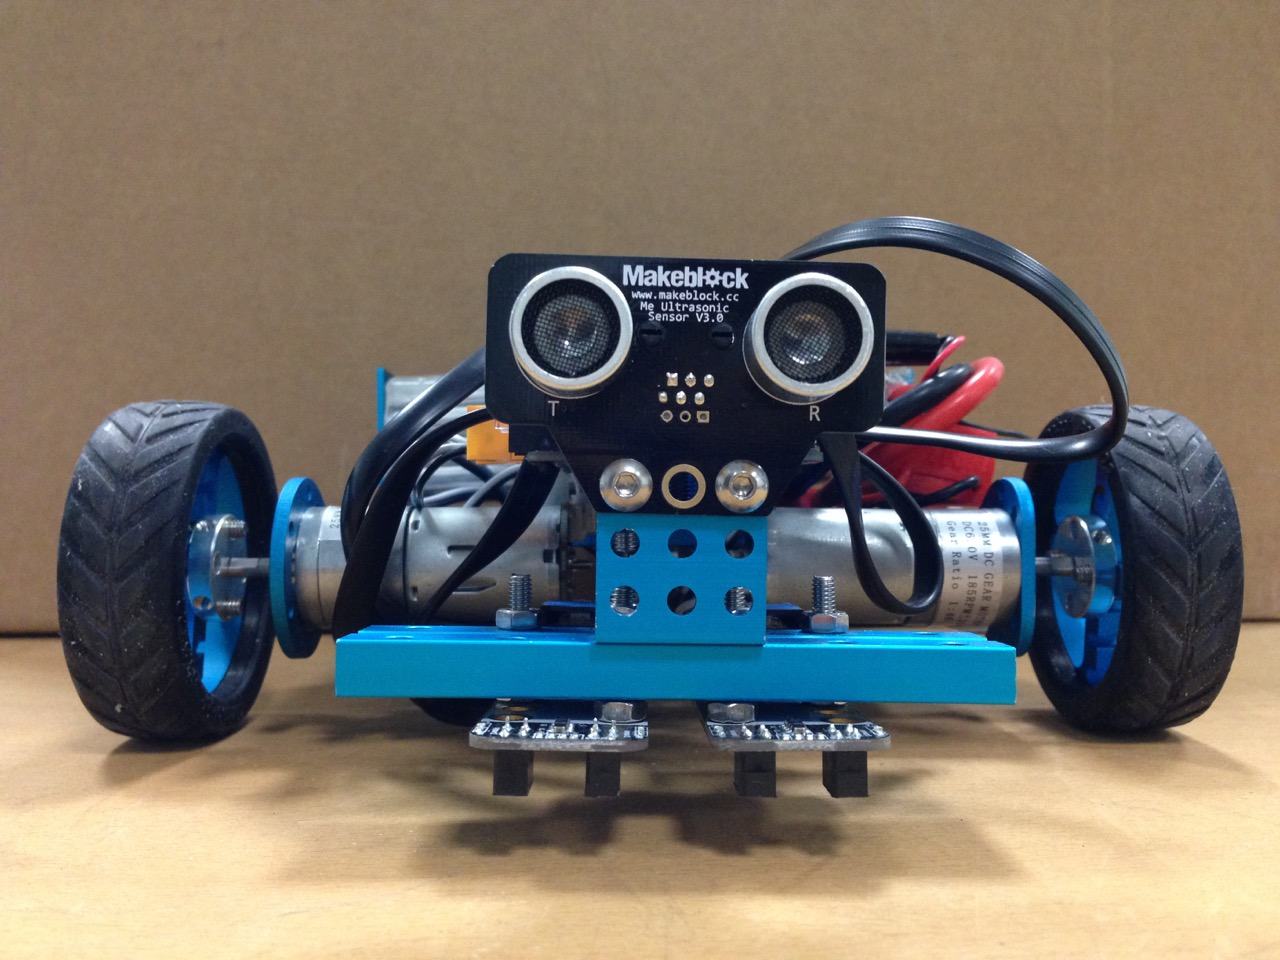
\includegraphics[width=.4\textwidth]{IMG_0759.jpg} }\quad
\subfloat[][\emph{scorcio}]{
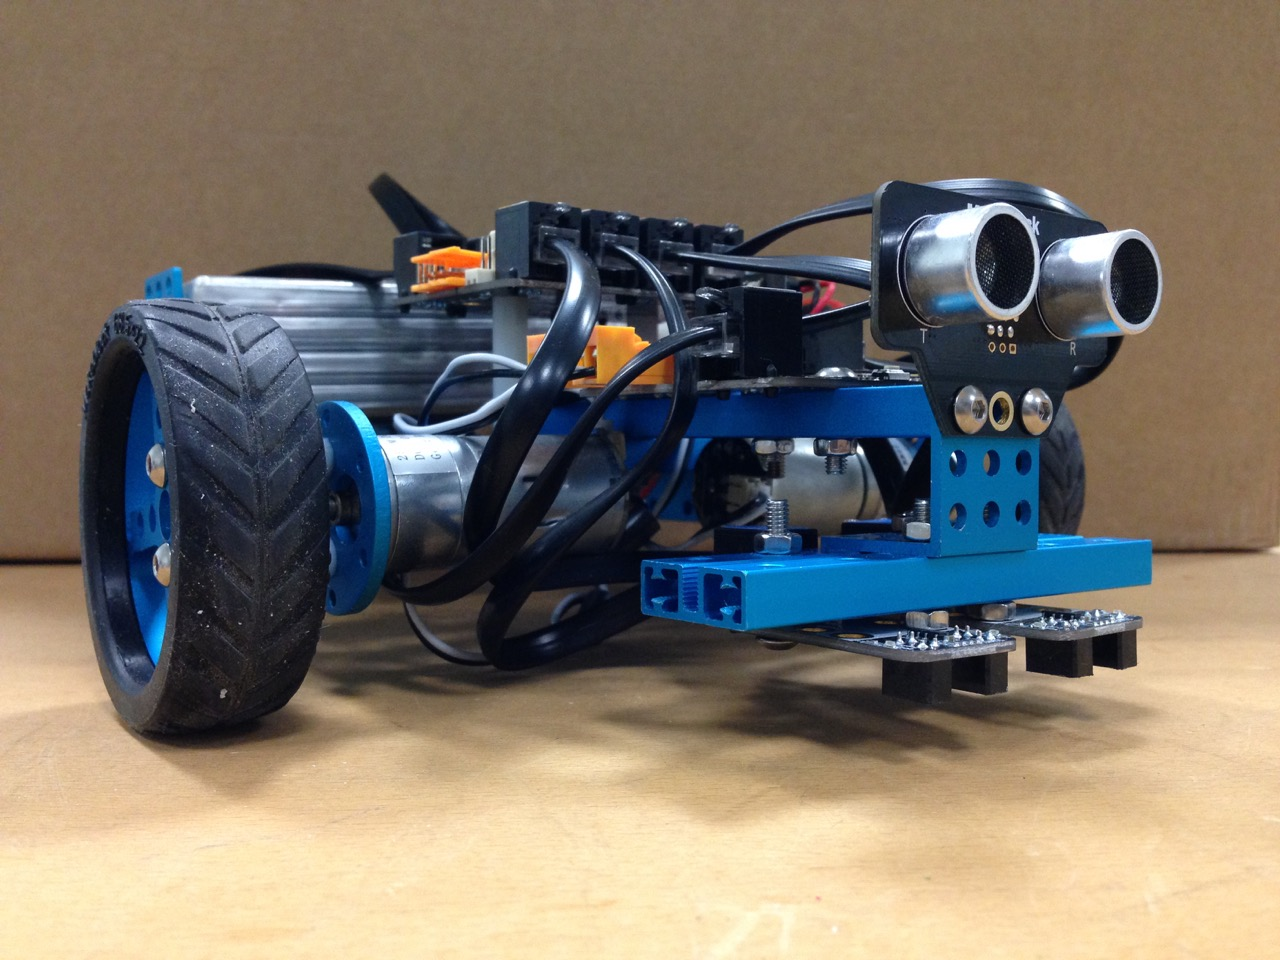
\includegraphics[width=.4\textwidth]{IMG_0763.jpg}}
\caption{Struttura robot}
\label{struct}
\end{figure}
\\La parte elettronica è basata sulla scheda MeOrion baseboard, un modulo a ultrasuoni per il rilevamento degli ostacoli, due moduli per i sensori tipo MeLineFollower, un modulo bluetooth. In figura \ref{schema} è illustrato il dettaglio dei collegamenti.
La scelta di adottare una coppia di sensori di linea è stata fatta per ottenere una migliore lettura del percorso, per una maggiore capacità di identificazione di casi particolari, come ad esempio curve a 90$^{\circ}$ o gli incroci e per un miglior controllo dei motori.
\begin{figure}[h]
	\subfloat[][\emph{collegamenti}]{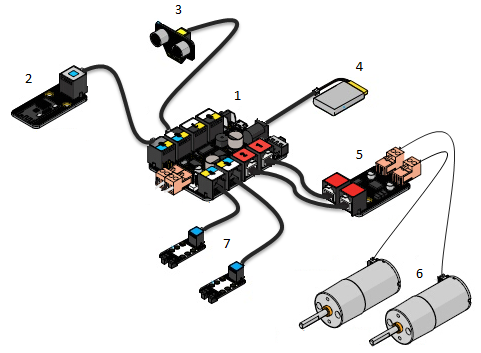
\includegraphics[width=.65\textwidth]{SCHEMA}}\quad
\subfloat[][\emph{lista dei compomenti}]{\begin{tikzpicture}[->, >=stealth', shorten >=1pt, auto, node distance=1cm, semithick]

%====Definizione stile stati================================================

	\tikzstyle{every state}=[fill, draw, white ,text=black]

%====Definizione stati e posizione===========================================

	\node[state](A) [label = 0:Me Orion ]                  			{1}; 	
 	\node[state](B) [below of= A, label = 0:Me Bluetooth]	{2};		
 	\node[state](C) [below of= B, label = 0:Line Follower]	{3};
  	\node[state](D) [below of= C, label = 0:Me Ultrasonic Sensor]{4};		
  	\node[state](E) [below of= D, label = 0:Batteria Li-Po]{5};	
  	\node[state](F) [below of= E, label = 0:Me Dual DC MotorDriver]{6};
  	\node[state](G) [below of= F, label = 0:Me DCMotor]{7};	
  	\end{tikzpicture}}
\caption{Componenti elettronici}
\label{schema}
\end{figure}		
\subsection{Software}
L'implementazione del software, basata sul C++, è il cuore del progetto. Ci si è avvalsi delle librerie proprietarie Makeblock, della classe macchina a stati finiti, precedentemente realizzata, e di metodi appositamente elaborati per una corretta gestione delle funzionalità richieste.